\documentclass{article}
\usepackage[utf8]{inputenc}
\usepackage[left=1cm,right=0.5cm,bottom=0.5cm,top=0.5cm]{geometry}
\usepackage{setspace}
\usepackage{graphicx}
\usepackage{amsmath}
\usepackage{graphbox}
\usepackage{enumitem}
\setstretch{0.8}
\setlist{nosep}

% 1 side of paper
\begin{document}
\begin{center}
    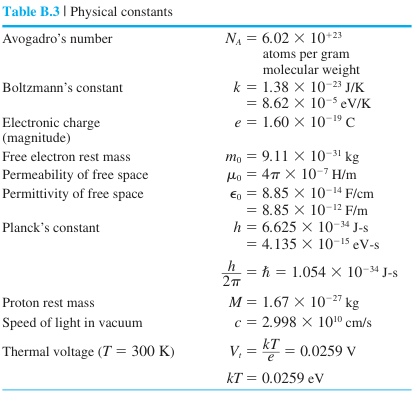
\includegraphics[align=c, height=7cm, width=4cm]{consts.png}
    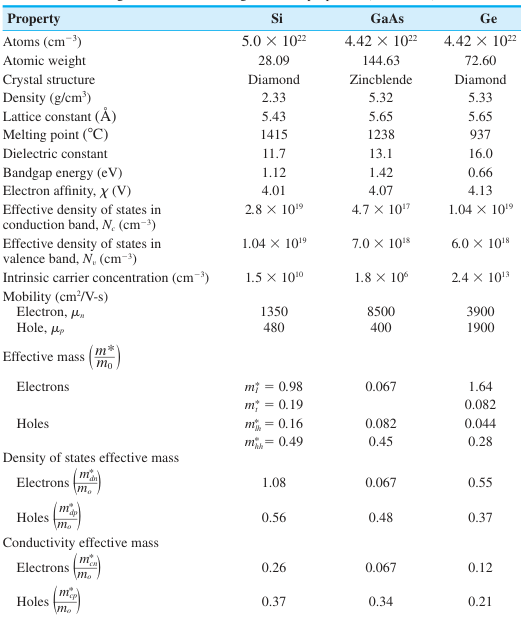
\includegraphics[align=c, height=7cm, width=4.5cm]{props.png}
    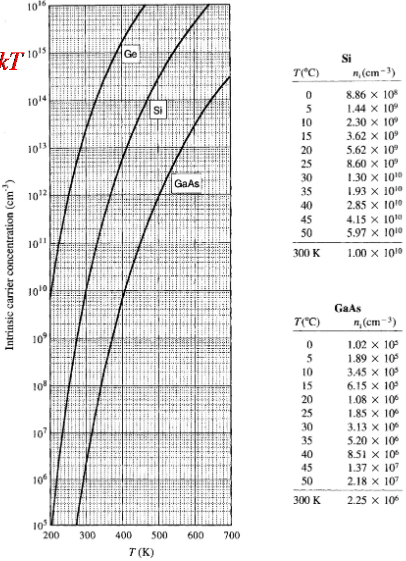
\includegraphics[align=c, height=7cm, width=4cm]{concentration.png}
    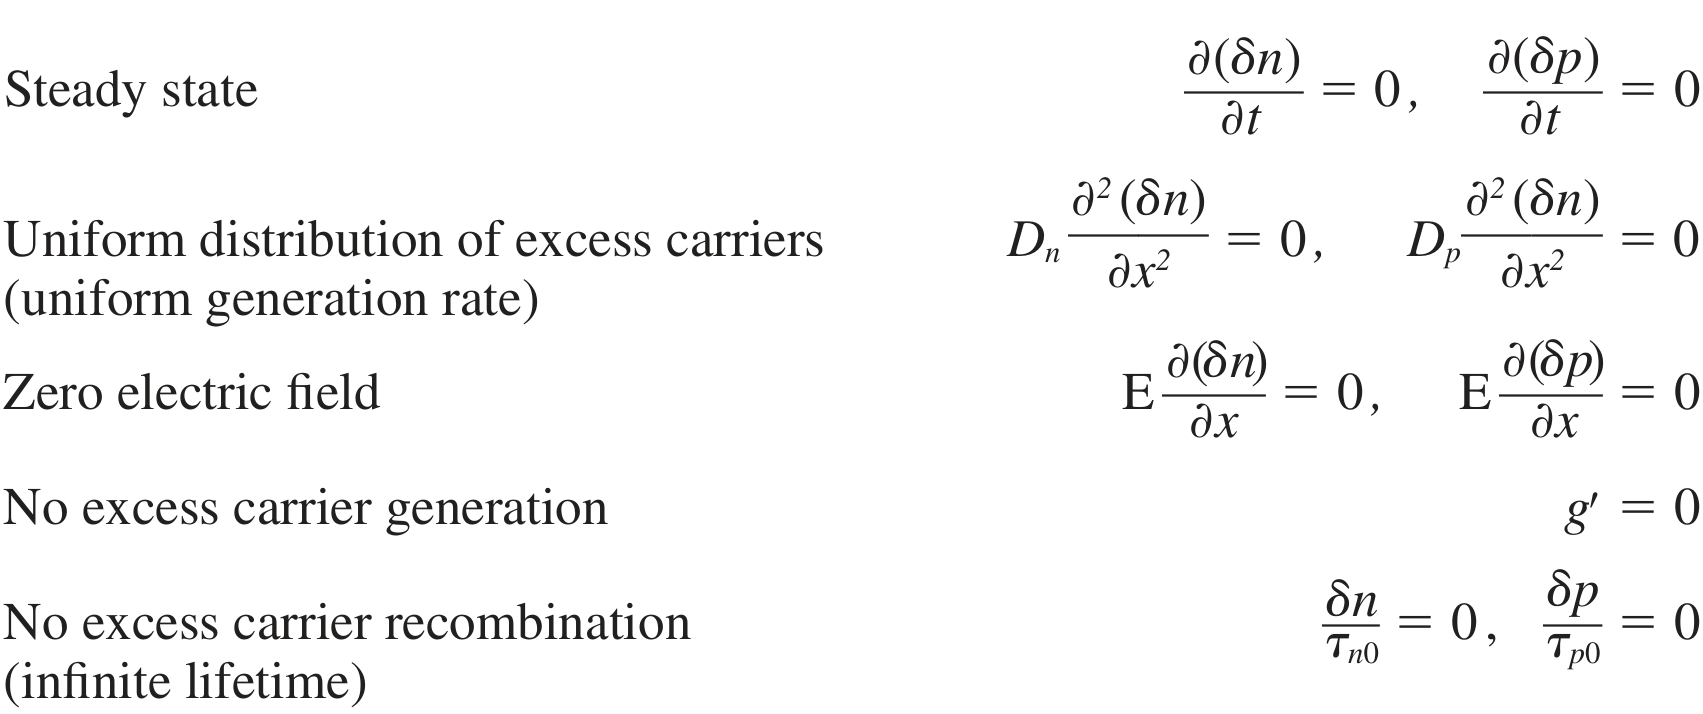
\includegraphics[align=c, height=7cm, width=7cm]{continuity.png}
\end{center}
% TODO: Chapter 1 concepts? Not many formulas up here, mostly concepts and geometry
\textbf{Basics of solids}
\begin{itemize}
    \item $E_c$ is the min energy of the conduction band, $E_v$ is the max energy of the valence band, $E_g$ is the bandgap ($E_c - E_v$)
    \item Density of states
    \begin{itemize}
        \item Conduction band: $g_c(E) = \frac{4 \pi (2m_n^*)^{3/2}}{h^3} \sqrt{E - E_c}$, Valence band: $g_v(E) = \frac{4 \pi (2m_p^*)^{3/2}}{h^3} \sqrt{E_v - E}$
    \end{itemize}
    \item Fermi-Dirac probability
    \begin{itemize}
        \item Probable distribution function: $f_F(E) = \frac{1}{1 + exp\left(\frac{E - E_F}{kT}\right)}$
        \item $f_F(E_F) = \frac{1}{2}$, and $E_F$ is known as the Fermi energy. Kind of the "center" of the distribution
        \item Boltzmann approx (when $E - E_F >> kT$): $f_F(E) \approx exp\left[\frac{-(E - E_F)}{kT}\right]$
    \end{itemize}
\end{itemize}
\textbf{Dopants}
\begin{itemize}
    \item Intrinsic means no dopants at all, extrinsic means doped. Complete ionization is assumed for all dopants.
    \item When $n_0 > p_0$, semiconductor is N-type (majority donors), and when $p_0 > n_0$, semiconductor is P-type (majority acceptors)
    \item Thermal equilibrium carrier concentrations
    \begin{itemize}
        \item Electron concentration (unit is $cm^{-3}$): $n_0 = N_c \cdot exp\left[\frac{-(E_c - E_F)}{kT}\right] = n_i \cdot exp\left[\frac{E_F - E_{Fi}}{kT}\right]$, $n_0 \propto N_c = 2\left(\frac{2 \pi m_n^* kT}{h^2}\right)^{3/2}$
        \item Hole concentration (unit is $cm^{-3}$): $p_0 = N_v \cdot exp\left[\frac{-(E_F - E_v)}{kT}\right] = p_i \cdot exp\left[\frac{-(E_F - E_{Fi})}{kT}\right]$, $p_0 \propto N_v = 2\left(\frac{2 \pi m_p^* kT}{h^2}\right)^{3/2}$
        \item $N_c$ and $N_v$ are the "effective density of states", and are \textbf{very temperature dependent} with $N = N_{T0} \cdot \frac{T}{T_0}^{3/2}$.
        \item For an intrinsic semiconductor, $n_i = p_i$, and $n_i^2 = N_c N_v exp\left[\frac{-E_g}{kT}\right] = N_c N_v exp\left[\frac{-(E_c - E_v)}{kT}\right]$
        \item For intrinsic AND extrinsic semiconductors, $n_0 \cdot p_0 = n_i^2$
    \end{itemize}
    \item Compensated semiconductors
    \begin{itemize}
        \item $n_0 = \frac{N_d - N_a}{2} + \sqrt{\left(\frac{N_d - N_a}{2}\right)^2 + n_i^2}$, $p_0 = \frac{N_a - N_d}{2} + \sqrt{\left(\frac{N_a - N_d}{2}\right)^2 + n_i^2}$
    \end{itemize}
    \item Fermi energy modelling
    \begin{itemize}
        \item For an intrinsic semiconductor, $E_{Fi} - E_{midgap} = \frac{3}{4} kT \ln \left(\frac{m_p^*}{m_n^*}\right)$
        \item We can use the $n_0$ functions: $E_c - E_F = kT \ln \left(\frac{N_c}{n_0}\right)$, $E_F - E_{Fi} = kT \ln \left(\frac{n_0}{n_i}\right)$ (n-type)
        \item We can use the $p_0$ functions: $E_F - E_v = kT \ln \left(\frac{N_v}{p_0}\right)$, $E_{Fi} - E_F = kT \ln \left(\frac{p_0}{n_i}\right)$ (p-type)
    \end{itemize}
\end{itemize}
\textbf{Carrier drift}
\begin{itemize}
    \item $J_{drf} = e(\mu_n n + \mu_p p)E = \sigma \cdot E$, $\rho = \frac{1}{\sigma} = \frac{1}{e(\mu_n n + \mu_p p)}$. N-type and P-type $n >> p$, $p >> n$ applies for simplification
    \item $J_{diff} = J_{n|diff} + J_{p|diff}$, $J_{n|diff} = e D_n \nabla{n} = e D_n \frac{dn}{dx}$ (in 2D), $J_{p|diff} = -e D_p \nabla{p} = -e D_p \frac{dp}{dx}$ (in 2D)
    \item $J = J_{drf} + J_{diff}$, $\frac{D_n}{\mu_n} = \frac{D_p}{\mu_p} = \frac{kT}{e}$, $\mu$ unit is $\frac{cm^2}{V \cdot s}$, $J$ unit is $\frac{A}{cm^2}$, $D$ unit is $\frac{cm^2}{s}$
    \item Flux is the true direction of electrons and holes. Current is opposite of flux for electrons, same for holes. Use flux for intuition
\end{itemize}
\textbf{Continuity equation}
\begin{itemize}
    \item Low injection means low number of excess carriers vs. equilibrium carriers
    \item P-type under low injection: $D_n \frac{\partial^2(\delta n)}{\partial x^2} + \delta n \mu_n \frac{\partial E}{\partial x} + \mu_n E \frac{\partial (\delta n)}{\partial x} + g' - \frac{\delta n}{\tau_{n0}} = \frac{\partial (\delta n)}{\partial t}$
    \item N-type under low injection: $D_p \frac{\partial^2(\delta p)}{\partial x^2} - \delta p \mu_p \frac{\partial E}{\partial x} - \mu_p E \frac{\partial (\delta p)}{\partial x} + g' - \frac{\delta p}{\tau_{p0}} = \frac{\partial (\delta p)}{\partial t}$
    \item $g'$ is generation, $\frac{\delta n}{\tau_{n0}}$ is recombination ($\tau_{n0}$ is the excess carrier lifetime), $D_n \dots$ is diffusion, $\mu_n E \dots$ is drift
    \item Case 1: Steady state with no additional carrier generation process and no drift ($g' = 0, \frac{\partial}{\partial t} = 0, E = 0$)
    \item Case 2: No drift and no carrier gradient ($\frac{\partial}{\partial x} = 0, E = 0$)
    \item Case 3: Steady state with no additional carrier generation process, no drift, no recombination ($g' = 0, \frac{\partial}{\partial t} = 0, E = 0, \tau_n \rightarrow \infty$)
    \item Case 4: No additional carrier generation process and uniform E field ($g' = 0, \frac{\partial E}{\partial x} = 0$)
\end{itemize}
\end{document}
